\chapter{Appendix}
\section{Source alignment}\label{sec:source-alignment}
\begin{figure}
	\centering
		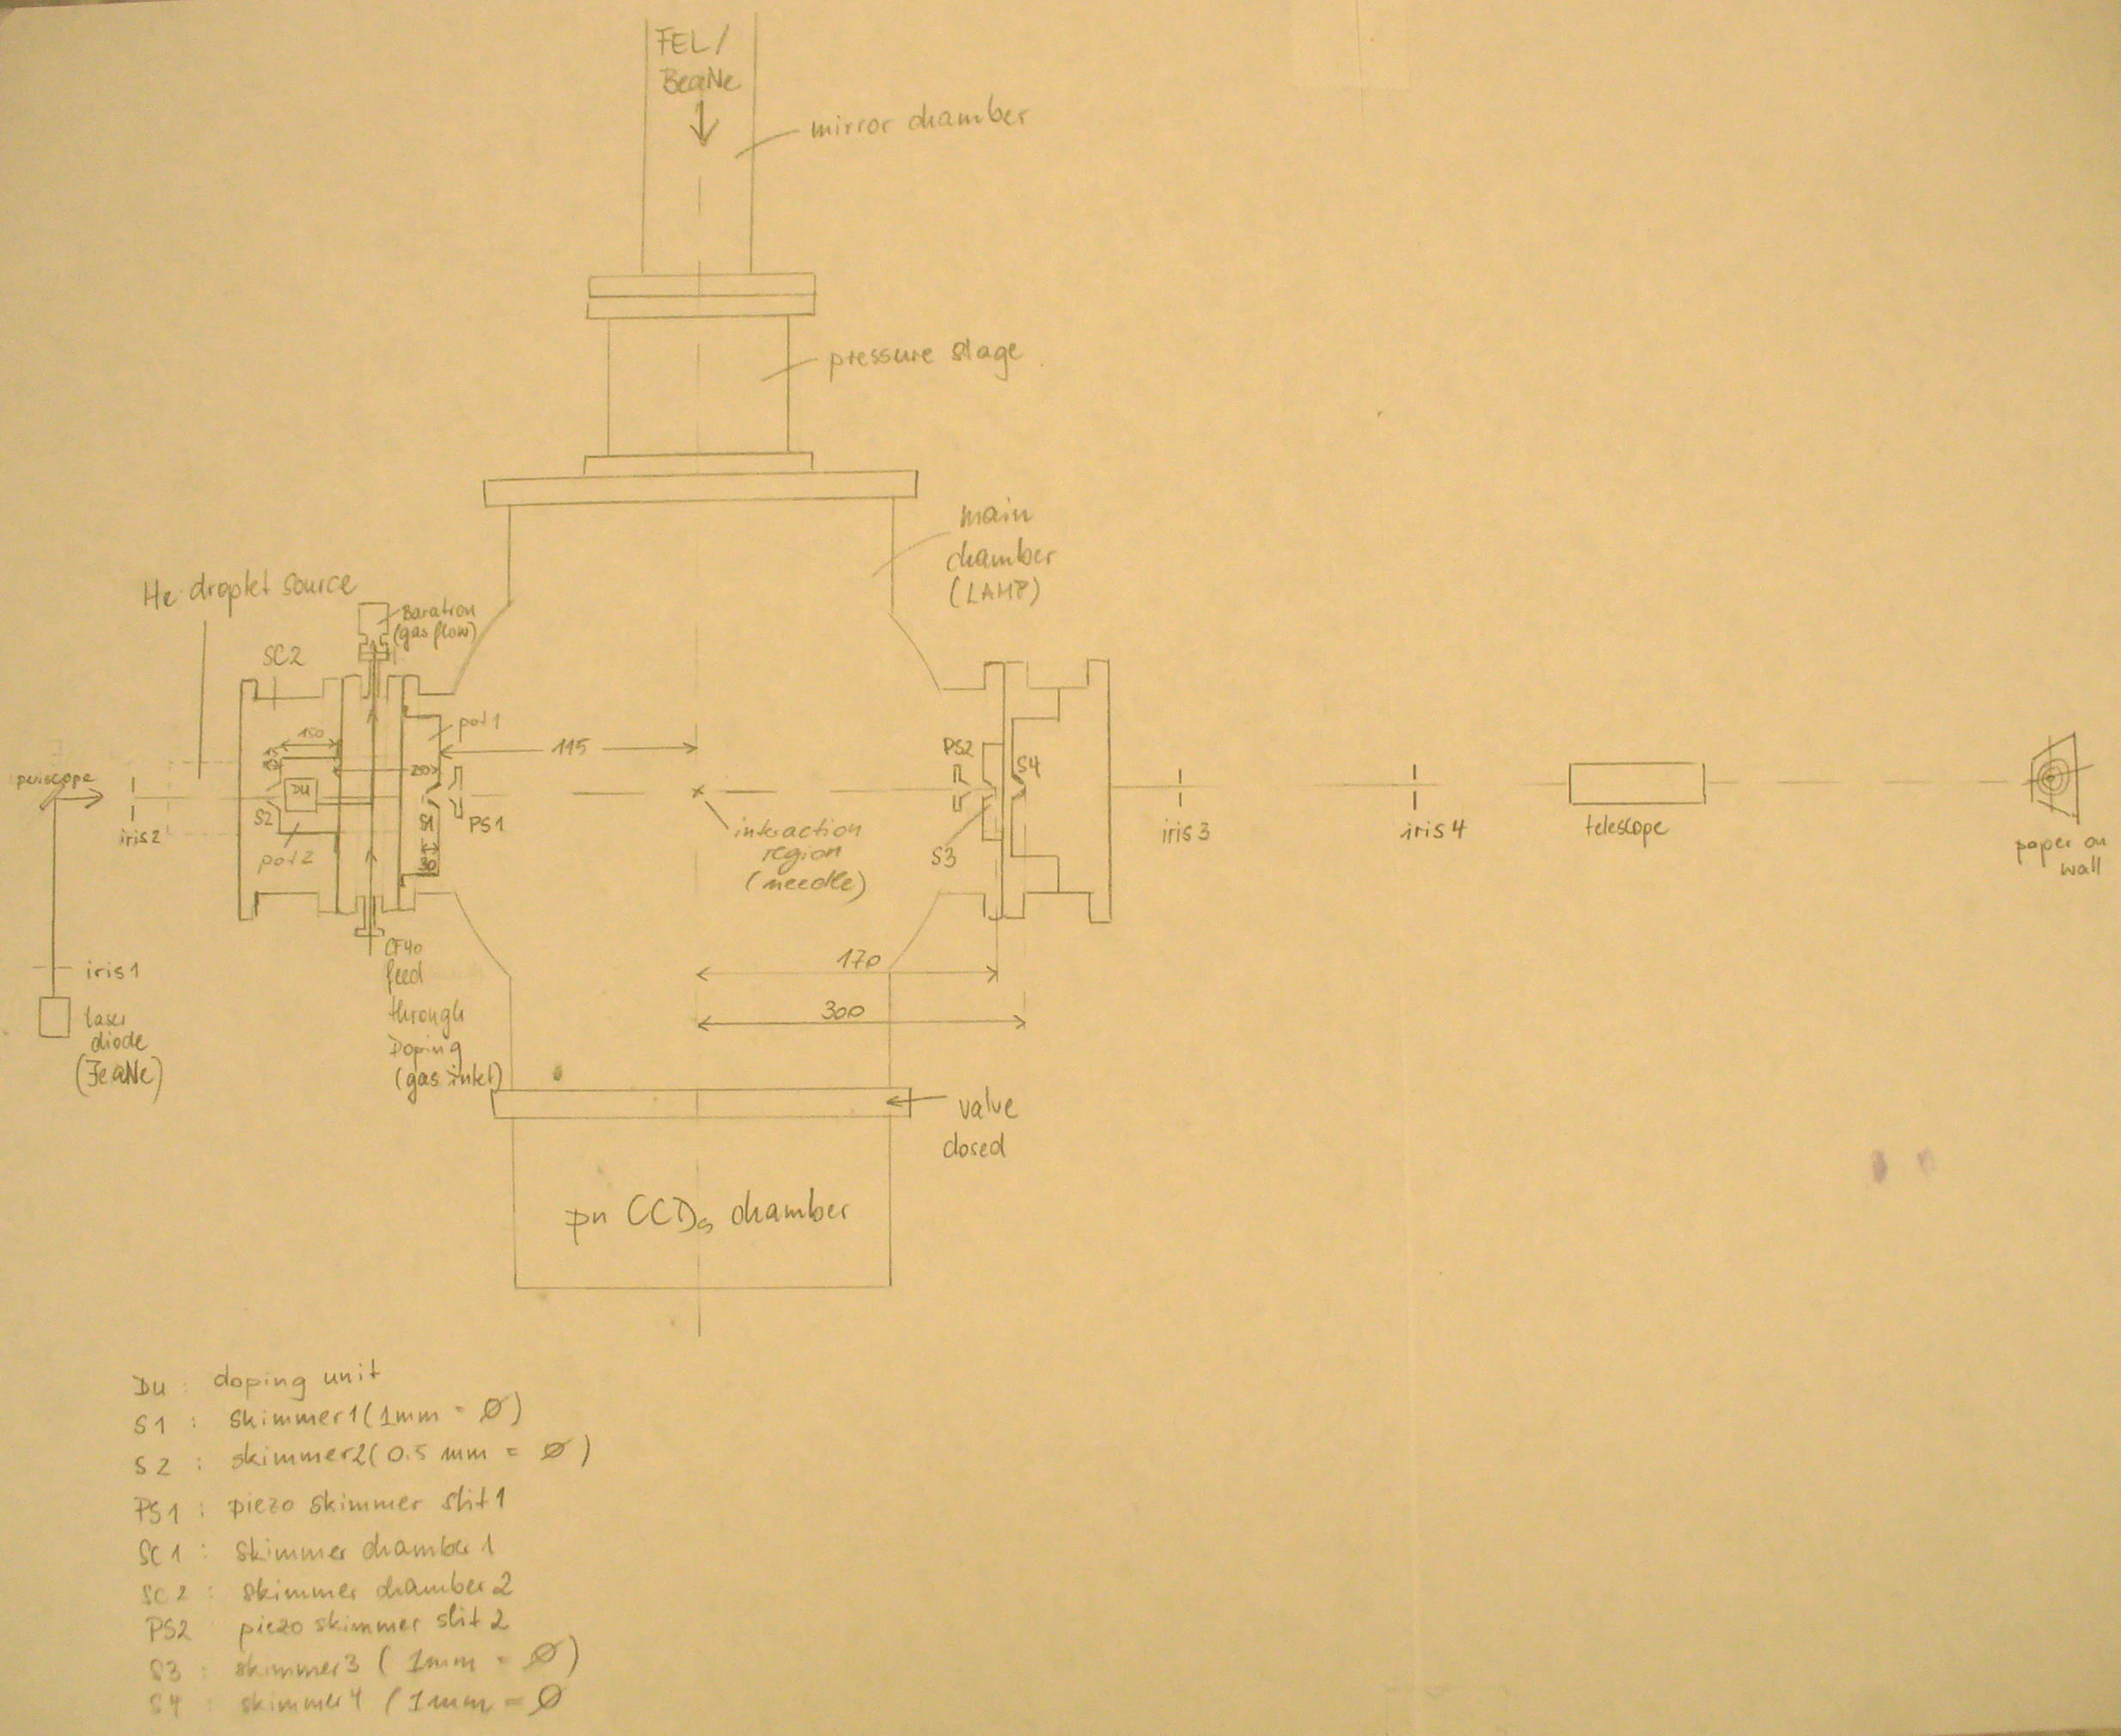
\includegraphics[width=1.00\textwidth]{images/Overview_Setup_Jetalignment.jpg}
	\caption{caption}
	\label{fig:Overview_Setup_Jetalignment}
\end{figure}
%
%
%
\section{Python code psana example}\label{sec:python-example}
Per popular request, a small analysis example is discussed\footnote{Programming languages change their syntax often, it is therefore useful to visit the web-page\\ \url{https://confluence.slac.stanford.edu/display/PSDM/LCLS+Data+Analysis}}. To begin, you should verify that you have a SLAC unix account and a SSH terminal with -Y flag capabilities\footnote{If you have problems with graphics visualization, try the following link\\ \url{https://confluence.slac.stanford.edu/display/PCDS/Remote+Visualization}}. To access the psana computer cluster, see the following commands
\begin{lstlisting}[language=csh]
	$ ssh -Y USERNAME@pslogin.slac.stanford.edu
	$ ssh -Y psana
	$ source /reg/g/psdm/etc/ana_env.csh
\end{lstlisting}
This logs you into the SLAC psana server and loads the psana framework. Once logged in, make yourself familiar with the following python code ‘psmonLocal.py’. ‘psmonLocal.py’ has been created by Chris O'Grady for demonstration purposes and more information can be found under\\
\url{https://confluence.slac.stanford.edu/display/PSDM/Visualization+Tools}
\lstinputlisting[language=Python,frame=single]{manuals/psmonLocal.py}
This script demonstrates a pixel detector image (CSpad) and an XY-Plot. Finally, run the script like any python script with
\begin{lstlisting}[language=csh]
	$ python /reg/g/psdm/tutorials/examplePython/psmonLocal.py
\end{lstlisting}
An interesting aspect to the python interaction is the 'TAB' method, where one can code without reading the documentation. Here a user should be on the psana servers and start ipython as follows
\begin{lstlisting}[language=csh]
	$ ipython
\end{lstlisting}
\begin{lstlisting}[language=Python]
	$ from psana import *
	$ ds = DataSource('exp=amotut13:run=206')
	$ det = Detector('AmoETOF.0:Acqiris.0')
	$ det.   (NOTE: user hits <TAB> after typing the "." to get list of available methods)
	$ evt = ds.events().next()    (NOTE: getting an event, since the above "Definition" line requires it)
	$ print det.waveform(evt)     (NOTE: calling the "waveform" method as required by the above "Definition" line)
\end{lstlisting}
TBD
%
%
%
\section{Python code on spherical integrations}
\section{Python code on combining detectors}